\documentclass[10pt]{article}
\usepackage[a4paper,margin=0.62in]{geometry}
\usepackage[T1]{fontenc}
\usepackage{lmodern}
\usepackage{graphicx}
\usepackage{xcolor}
\usepackage{booktabs}
\usepackage{tabularx}
\usepackage{enumitem}
\usepackage{hyperref}
\usepackage{caption}
\usepackage{float}

\definecolor{reportblue}{HTML}{174A7C}
\definecolor{muted}{HTML}{4A5568}
\hypersetup{colorlinks=true,linkcolor=reportblue,urlcolor=reportblue}
\setlist[itemize]{leftmargin=1.2em,itemsep=0.15em,topsep=0.15em}
\setlist[enumerate]{leftmargin=1.35em,itemsep=0.15em,topsep=0.15em}
\captionsetup{font=small,labelfont=bf}
\renewcommand{\arraystretch}{1.12}
\setlength{\parindent}{0pt}
\setlength{\parskip}{0.45em}

\title{\vspace{-2.8em}\textbf{Illegal Brick Kiln Detector}\\
\large AI-assisted satellite review for environmental monitoring in Bangladesh}
\author{Team PTSD\\AI Hackathon SciBlitz AI Challenge 2026\\
\small Samonwita Sarker (Leader), Protik Dev, Rotna Dipika Debnath, Touhidul Alam Seyam}
\date{July 2026}

\begin{document}
\maketitle
\vspace{-1.4em}

\textbf{Summary.} Illegal Brick Kiln Detector is a map-first web app for finding likely brick kilns in satellite tiles. It uses a fine-tuned YOLO11n-OBB model, served through a Python prediction endpoint, and a Next.js dashboard for review. The reviewer sees the tile, class, confidence, location, and oriented box before deciding whether a detection is worth follow-up.

\section{Problem statement}
Brick kilns are a local pollution and land-use problem in Bangladesh. They are spread across many districts, and in satellite images they can look similar to other industrial or rural structures. Manual review takes time, especially when a reviewer has to move between maps, image crops, and notes.

A useful tool cannot just say "kiln" or "no kiln." It has to show where the object is, how confident the model is, and what image evidence the model used. This project targets environmental analysts, civil-society monitors, and government reviewers who need a faster way to triage suspected kilns before any field check or enforcement step.

\section{Proposed solution}
The project is an AI-assisted dashboard for district-level kiln review. A reviewer selects a district, runs prediction on seeded satellite tiles, then reviews the detections on a map and in a list. Each detection includes latitude, longitude, kiln class, confidence, source tile, and an oriented bounding box in the detail view.

\begin{figure}[H]
  \centering
  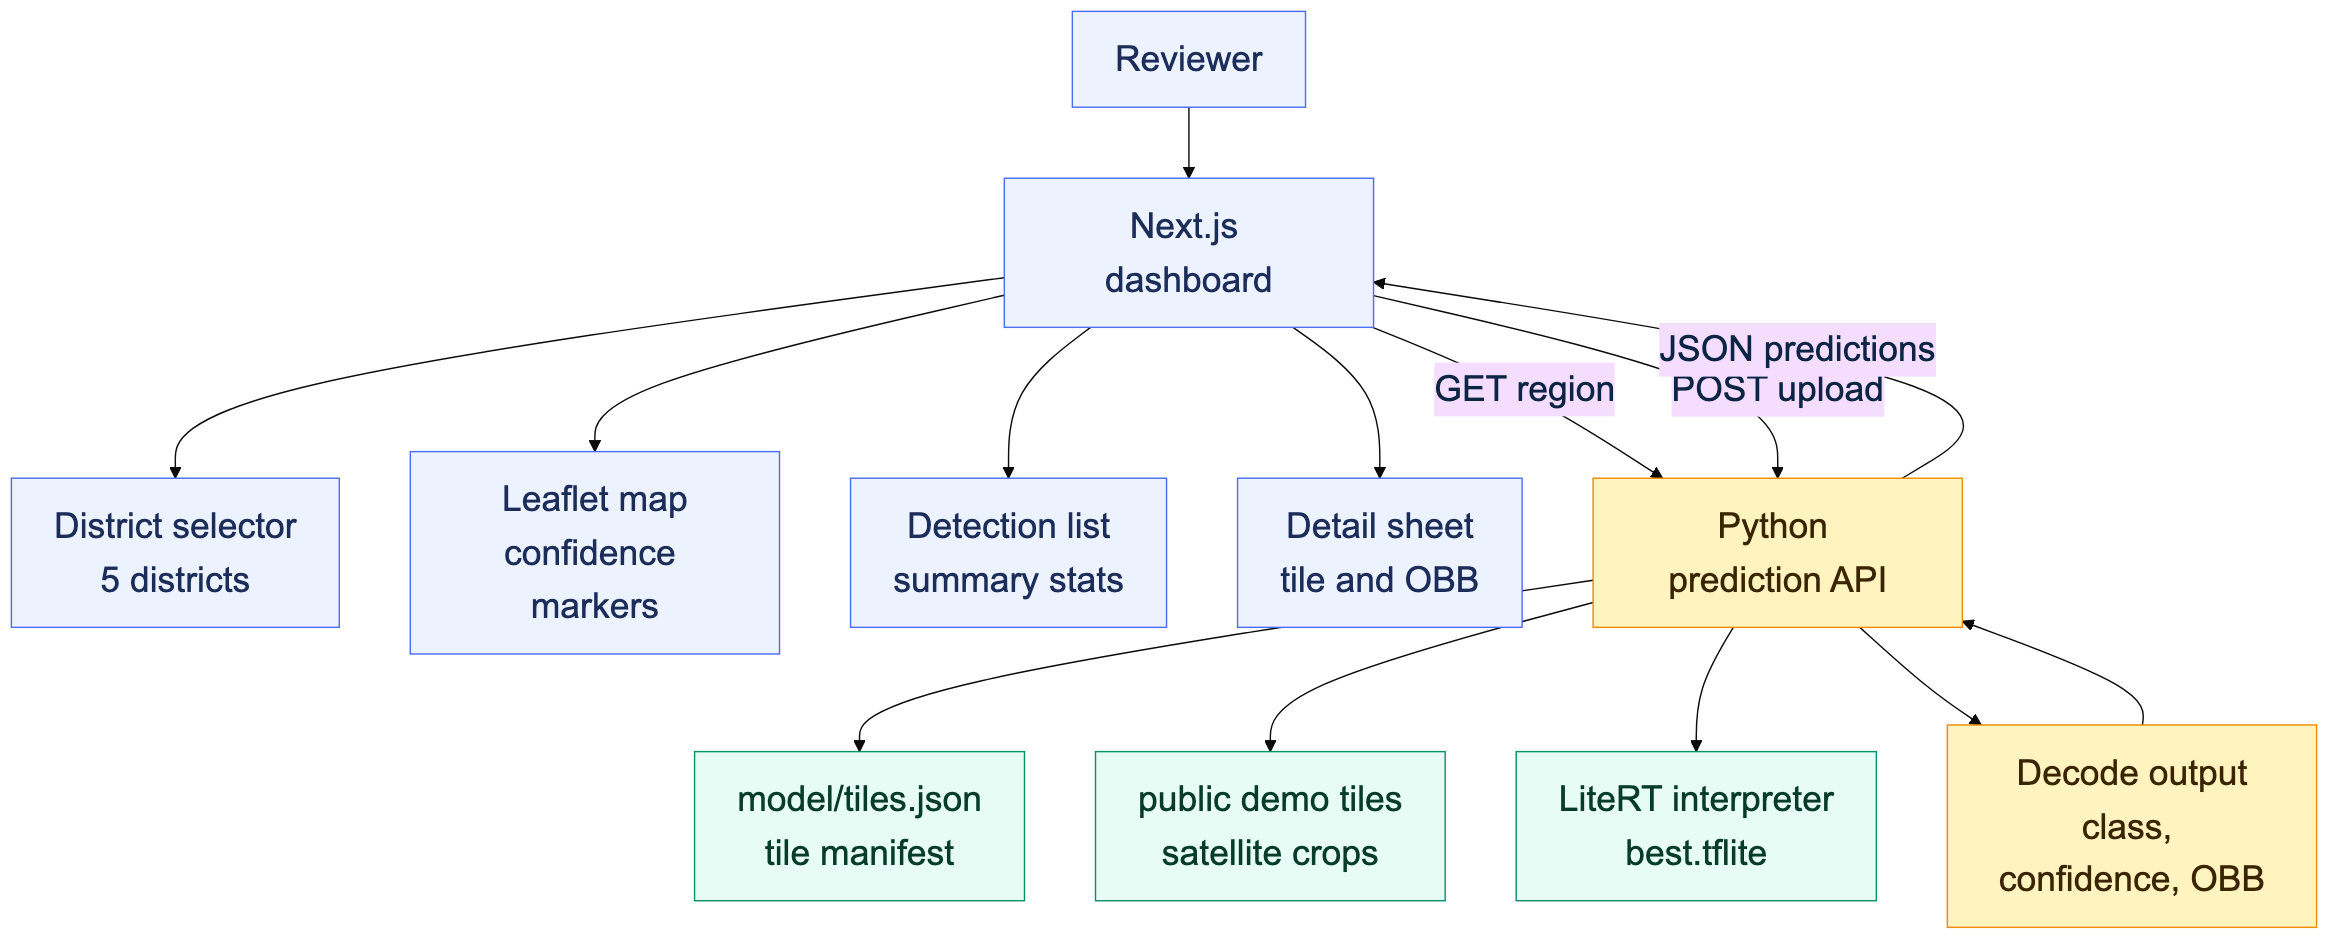
\includegraphics[width=0.95\linewidth]{diagrams/app-architecture.png}
  \caption{Application architecture for the dashboard, prediction API, model file, tile manifest, and review UI.}
\end{figure}

The diagram separates the user interface from the model-serving layer. The dashboard handles district selection, map review, detection lists, and the detail sheet. The Python API loads seeded tiles or uploaded images, runs the LiteRT model, decodes the oriented boxes, and sends structured JSON back to the UI.

\textbf{Implemented product surface.}
\begin{itemize}
  \item Next.js App Router dashboard with shadcn/ui components and Leaflet mapping.
  \item Python \texttt{/predict} API supporting seeded region prediction and transient image upload prediction.
  \item LiteRT/TFLite model artifact at \texttt{model/best.tflite} for local or Vercel-style Python serving.
  \item Five supported Bangladesh districts: Brahmanbaria, Jessore, Manikganj, Mymensingh, and Tangail.
  \item Fifty bundled demo tiles, ten per district, listed in \texttt{model/tiles.json} and served from \texttt{public/demo-tiles/}.
\end{itemize}

\section{Methodology}
The training workflow is in \texttt{yolo-obb-n (1).ipynb}. The app workflow is in the prediction API, typed frontend parser, region helpers, and dashboard components in this repository.

\begin{figure}[H]
  \centering
  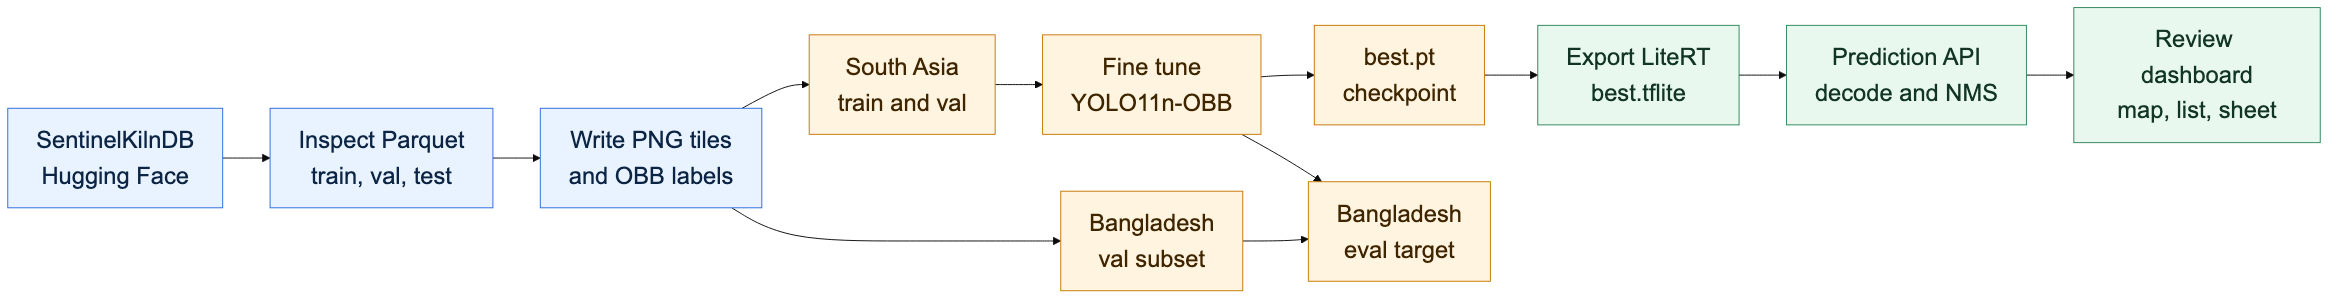
\includegraphics[width=\linewidth]{diagrams/ml-pipeline.png}
  \caption{Training and deployment path from SentinelKilnDB to the LiteRT model used by the app.}
\end{figure}

The pipeline starts with SentinelKilnDB Parquet files and turns them into YOLO-OBB training data. The model is trained on the wider South Asia split, while the Bangladesh subset is kept for regional evaluation. The trained \texttt{best.pt} checkpoint is then exported to \texttt{best.tflite} so the app can run inference through a lighter Python API.

\textbf{Data preparation.} The notebook downloads SentinelKilnDB from the Hugging Face dataset repository SustainabilityLabIITGN/SentinelKilnDB. It reads the train, validation, and test Parquet files, extracts PNG tile images, and writes YOLO-OBB label files. The final class order is \texttt{CFCBK}, \texttt{FCBK}, and \texttt{Zigzag}.

\textbf{Training split and regional evaluation target.} The notebook trains on the full South Asia split instead of Bangladesh only. That gives the model more kiln examples and keeps the rare CFCBK class from becoming too small. It also creates a Bangladesh validation subset from latitude 20.5 to 26.7 and longitude 88.0 to 92.7.

\textbf{Product workflow.} Predictions are transient. The dashboard requests them, renders markers and list rows, and opens a detail sheet for visual review. Upload prediction accepts an image data URL in memory and does not save the image.

\section{AI/ML approach}
The detector starts from the pretrained Ultralytics \texttt{yolo11n-obb.pt} checkpoint and fine-tunes it for oriented object detection. Oriented boxes matter here because kilns are often long, narrow, and rotated inside the tile. The deployed model predicts CFCBK, FCBK, and Zigzag.

\begin{table}[H]
  \centering
  \small
  \begin{tabularx}{\linewidth}{@{}lX@{}}
    \toprule
    Item & Value from notebook or repository \\
    \midrule
    Base model & \texttt{yolo11n-obb.pt}, pretrained Ultralytics YOLO OBB model \\
    Task & Oriented object detection for brick kiln classes \\
    Dataset & SentinelKilnDB, downloaded from Hugging Face \texttt{SustainabilityLabIITGN/SentinelKilnDB} \\
    Image size & 128 px training and validation tiles in the completed notebook run \\
    Epochs & 50 completed epochs \\
    Batch & 256 on Kaggle GPU environment \\
    Device & Kaggle CUDA run with Tesla T4 GPUs shown in notebook output \\
    Augmentation & 90 degree rotation, horizontal and vertical flips, scale, translate, mosaic, cosine LR \\
    Export & \texttt{model/best.pt} to LiteRT/TFLite \texttt{model/best.tflite}; expected shape input \texttt{(1,3,256,256)}, output \texttt{(1,8,1344)} \\
    \bottomrule
  \end{tabularx}
  \caption{Model and training configuration.}
\end{table}

The Python API converts each image to RGB, resizes it to the model input size, normalizes pixels, runs the LiteRT interpreter, decodes YOLO OBB output, filters by confidence, applies NMS, maps tile coordinates to latitude and longitude, and returns JSON to the frontend.

\section{Results}
The completed notebook run extracted 71,856 training tiles and 23,952 validation tiles. Ultralytics reported 24,642 training background images and 8,214 validation background images during label scanning. The Bangladesh validation subset contained 3,929 tiles. The saved notebook output includes final overall validation metrics, but not a separate final Bangladesh-only table, so this report treats that subset as an evaluation target rather than a reported score.

\begin{table}[H]
  \centering
  \small
  \begin{tabular}{@{}lrrrrrr@{}}
    \toprule
    Class & Images & Instances & Precision & Recall & mAP50 & mAP50-95 \\
    \midrule
    All & 23,952 & 21,042 & 0.651 & 0.627 & 0.643 & 0.359 \\
    CFCBK & 587 & 649 & 0.661 & 0.572 & 0.592 & 0.374 \\
    FCBK & 9,010 & 11,339 & 0.618 & 0.672 & 0.634 & 0.330 \\
    Zigzag & 7,110 & 9,054 & 0.675 & 0.636 & 0.702 & 0.375 \\
    \bottomrule
  \end{tabular}
  \caption{Final validation metrics recorded in the notebook output for \texttt{best.pt}.}
\end{table}

\textbf{System results.} The repository has a working prediction API contract and frontend parser. A region request returns \texttt{region}, \texttt{generatedAt}, and predictions with \texttt{id}, latitude, longitude, confidence, label, tile URL, optional class name, and optional OBB points. The UI summarizes total detections, confidence bands, average confidence, and per-class counts.

\begin{figure}[H]
  \centering
  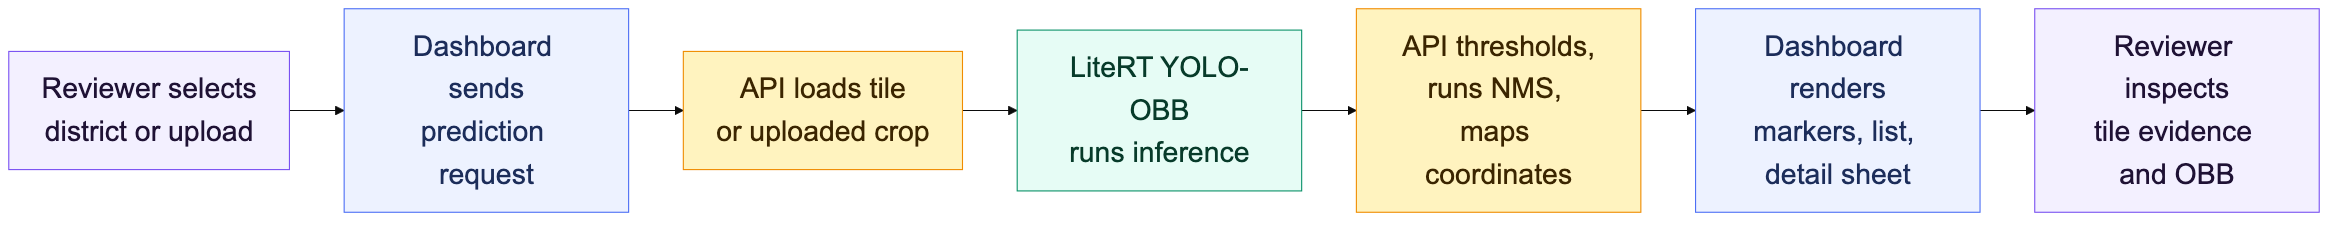
\includegraphics[width=0.96\linewidth]{diagrams/review-flow.png}
  \caption{Reviewer interaction sequence from district selection to evidence inspection.}
\end{figure}

This flow follows one review run. The reviewer starts with a district or upload, the frontend calls \texttt{/predict}, the API loads image evidence and runs model inference, then the decoded predictions return to the dashboard. The reviewer sees the result as map markers, list rows, and a detail sheet rather than a raw model response.

\section{Limitations and future work}
\textbf{Current limitations.}
\begin{itemize}
  \item The demo uses fifty bundled tiles and does not yet scan arbitrary large satellite mosaics.
  \item The available notebook output reports overall validation metrics, while Bangladesh-specific final metrics were not present in the saved cell outputs.
  \item Uploaded image predictions are transient and use reference tile metadata for approximate coordinates when the upload has no georeference.
  \item The API uses axis-aligned IoU during NMS even though the model predicts oriented boxes. This is practical, but it can handle edge cases imperfectly.
  \item There is no durable review database, audit log, reviewer feedback loop, or active-learning queue yet.
\end{itemize}

\textbf{Future work.}
\begin{itemize}
  \item Add a geospatial tiling pipeline for wider Bangladesh coverage and scheduled scans.
  \item Report Bangladesh-only precision, recall, mAP, and confusion analysis as a required evaluation artifact.
  \item Add reviewer feedback persistence so confirmed false positives and true positives can improve future training.
  \item Calibrate thresholds by district or kiln class. Triage may need higher recall, while enforcement review needs higher precision.
  \item Add exportable evidence bundles with source tiles, OBB overlays, and metadata.
\end{itemize}

\textbf{Reproducibility.} Install app dependencies with \texttt{bun install}. Run local development with \texttt{bun run dev} for Next.js and \texttt{python api/predict.py} for the prediction endpoint. The notebook writes \texttt{/kaggle/working/best.pt}; the export script converts it to \texttt{model/best.tflite}. Validate with \texttt{bun run lint} and \texttt{bun run build}.

\end{document}
